\subsection{Distancia promedio recorrida por los usuarios.}

Los datos abiertos contiene la localización geográfica de cada estación de MiBici. Para calcular entre estaciones se uso la ecuación \ref{eq:distance}.

\begin{equation}
    \begin{matrix}
        \beta = sin^2\left ( \frac{|\Delta \theta|}{2} \right ) + cos \left (\theta_1\right )  cos(\theta_2)sin^2 \left (\frac{|\Delta \phi|}{2} \right ) \\
        D     = 2R\;arcsin\left (\sqrt{\beta} \right )
    \end{matrix}
    \label{eq:distance}
\end{equation}

donde R es el radio de la tierra, $\theta_i$ es la latitud y $\phi_i$ es la longitud.

En base a las distancias calculadas en cada viaje realizado en el periodo 2015 al 2018. El calculo del promedio mensual por hora de las distancias recorridas en cada viaje se realizó con la ecuación \ref{eq:monthly_hourly_mean_distance}.

\begin{equation}
    \bar{D}_{m,h} = \frac{1}{n_{(m,h)}} \sum_{i=1}^{n_{(m,n)}} \hat{D}_{i} \qquad \begin{matrix}
        m=1,2,\dots,12 \\ h=6,7,\dots,23
    \end{matrix} \label{eq:monthly_hourly_mean_distance}
\end{equation}

donde $\hat{D}$ y $n_{(m,n)}$ es el conjunto y la cantidad total de viajes realizados para el mes $m$ realizados entre las $h$ y $h+1$ horas respectivamente. De una manera semejante, se calculo la varianza de este conjunto con la ecuación \ref{eq:monthly_hourly_var_distance}.

\begin{equation}
    \sigma_{D_{(m,h)}} = \frac{1}{n_{(m,h)}-1} \sum_{i=1}^{n_{(m,n)}} (D_i-\bar{D}_{(m,h)})^2 \qquad \begin{matrix}
        m=1,2,\dots,12 \\ h=6,7,\dots,23
    \end{matrix} \label{eq:monthly_hourly_var_distance}
\end{equation}

En la figura \ref{fig:monthly_hourly_distance} se muestran los resultados de aplicar las ecuaciones \ref{eq:monthly_hourly_mean_distance} y \ref{eq:monthly_hourly_var_distance} a los datos de las distancias.

En la figura \ref{fig:monthly_hourly_mean_distance} se visualiza que existe una disminución de su uso entre las 10 y 16 horas a lo largo del año y entre los meses mayo y julio en cualquier horario. Este último coincide con la temporada del año donde se presentan más lluvias\cite{clima_guadalajara}. Con esto, tenemos que existe un mínimo de la distancia recorrida entre las 14 y 16 horas en los meses de junio y julio. Con ayuda de la figura \ref{fig:monthly_hourly_var_distance} se obtiene que la distancia recorrida por los usuarios entre los meses de septiembre y diciembre tienen una mayor variación y esto puede deberse a la baja temperatura\cite{clima_guadalajara}. Ya que los usuarios al sentir menos sudor al usar la bicicleta como transporte pueden ir más calmados en sus trayectos.

\begin{figure}[H]
    \centering
    \begin{subfigure}[b]{8cm}
        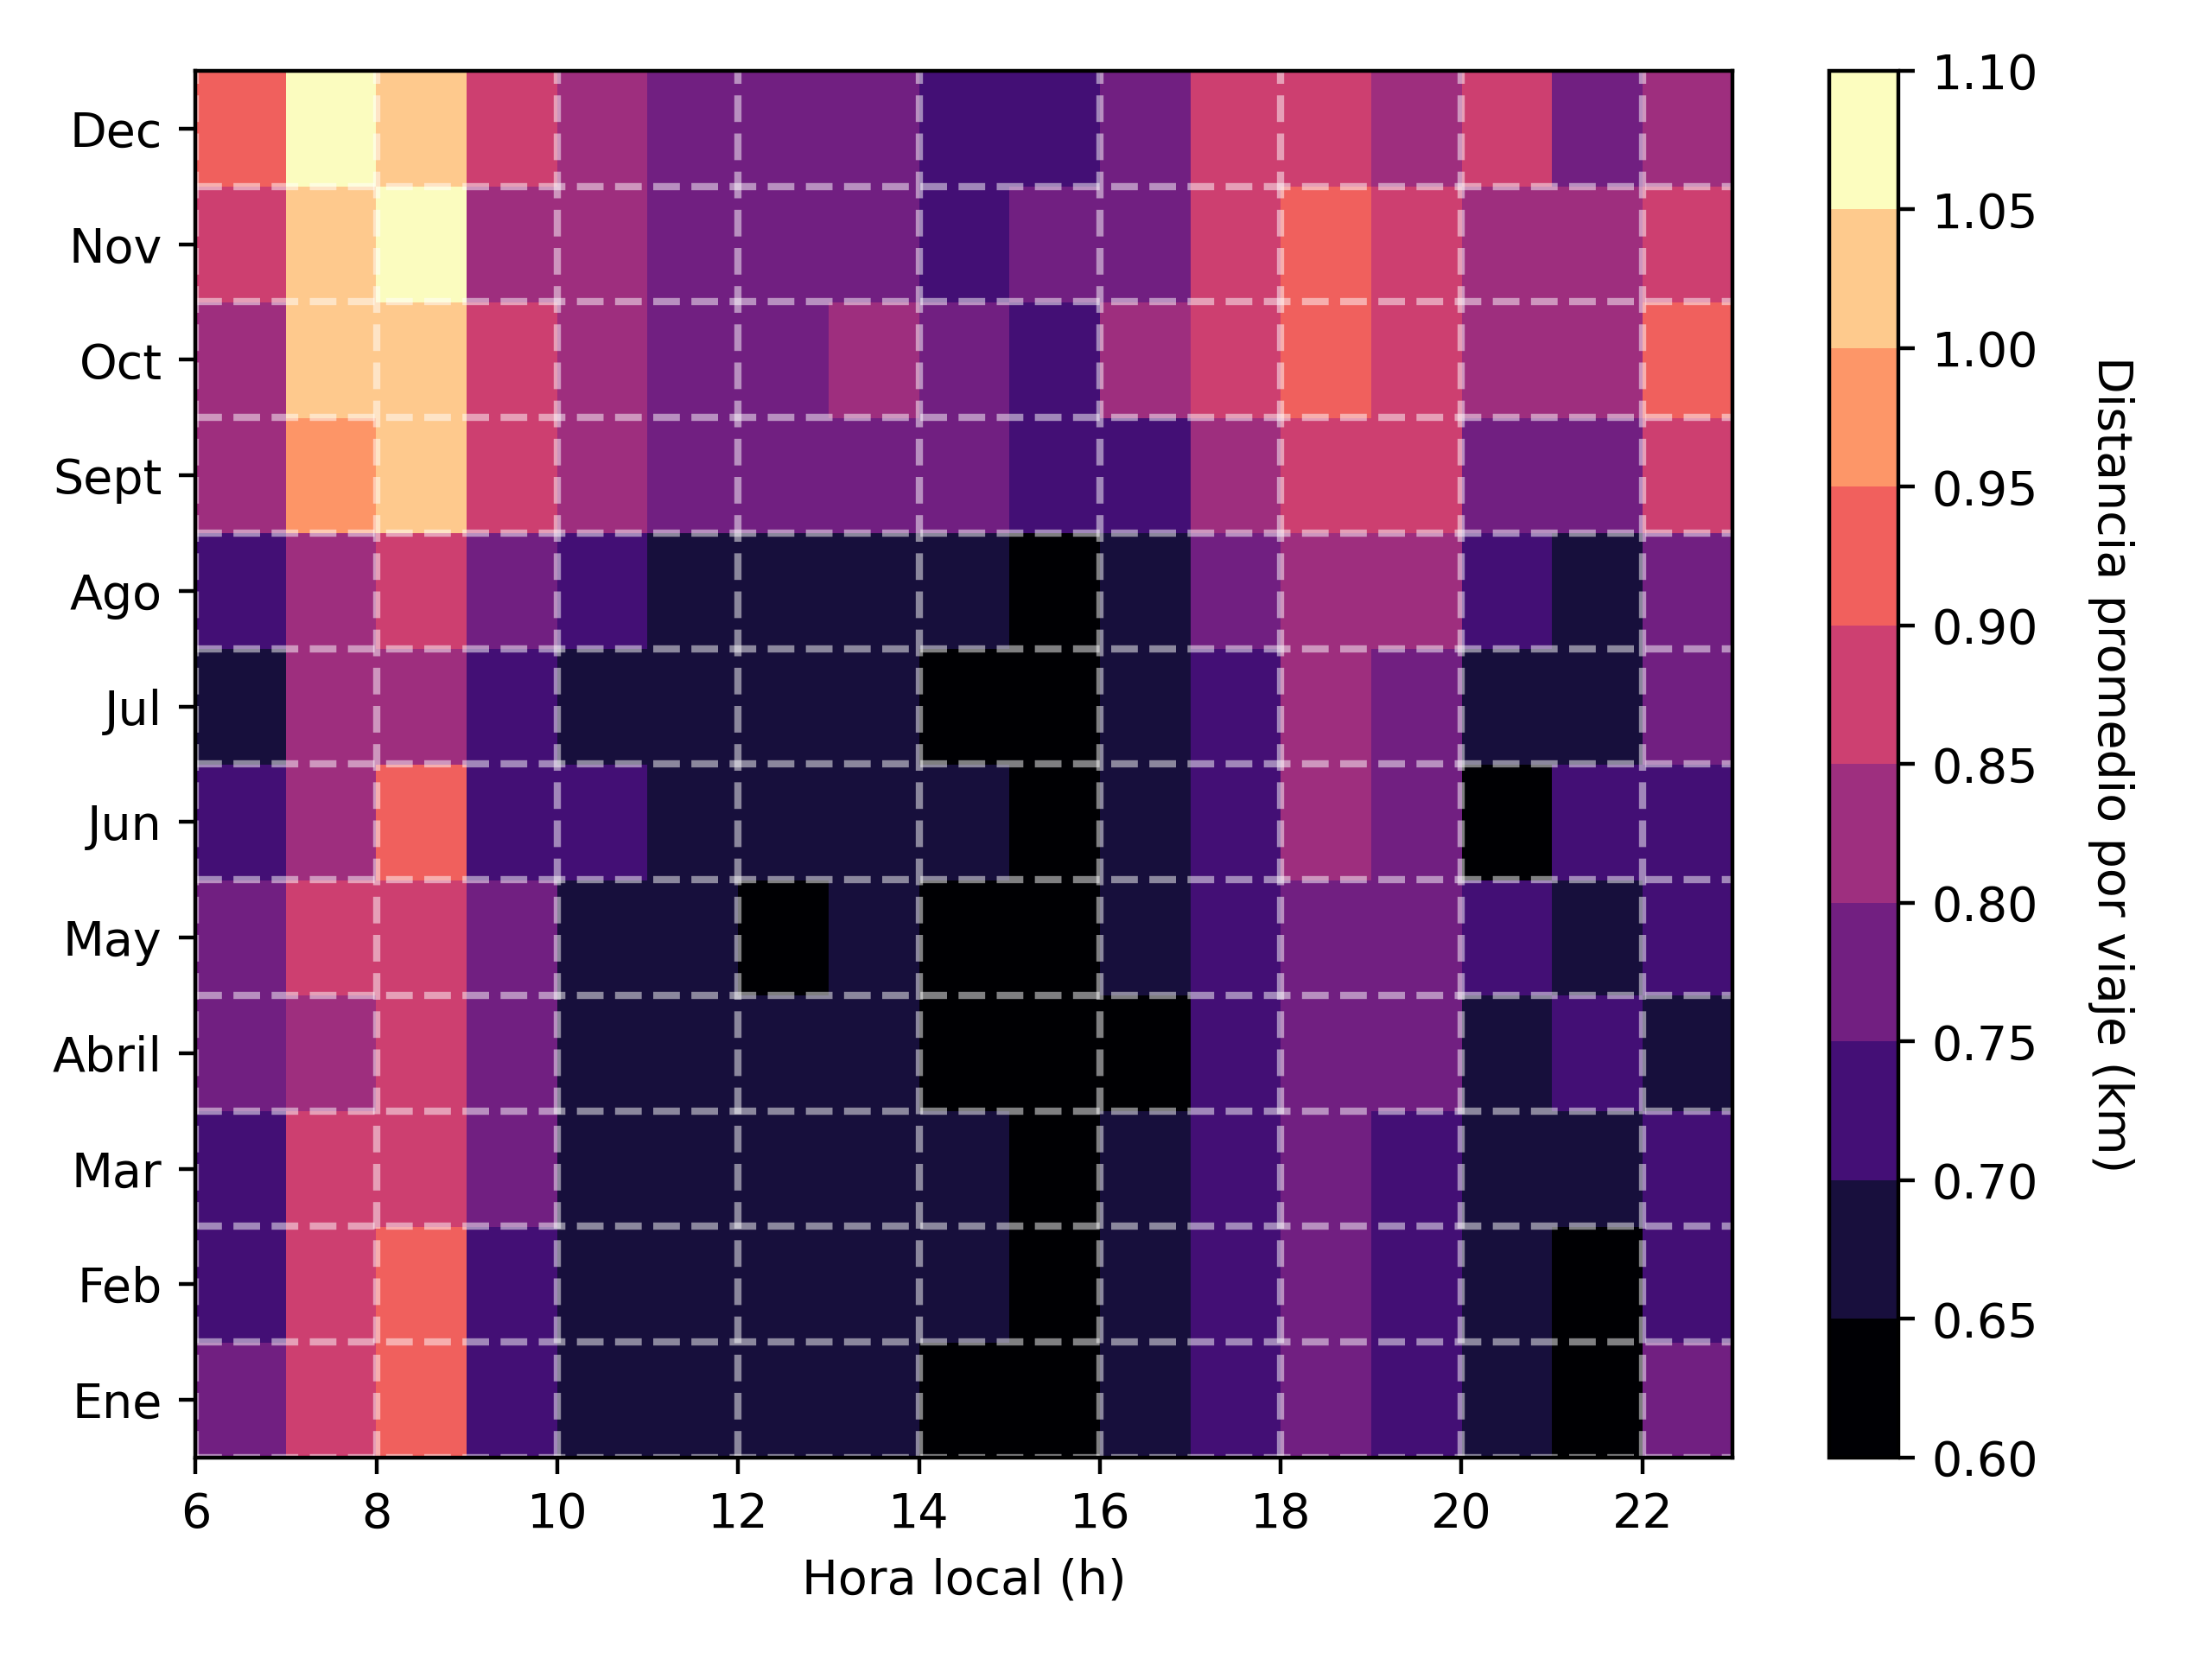
\includegraphics[width=8cm]{Graphics/monthly_hourly_mean_distance.png}
        \caption{Promedio mensual de la distancia recorrida.}
        \label{fig:monthly_hourly_mean_distance}
    \end{subfigure}
    \begin{subfigure}[b]{8cm}
        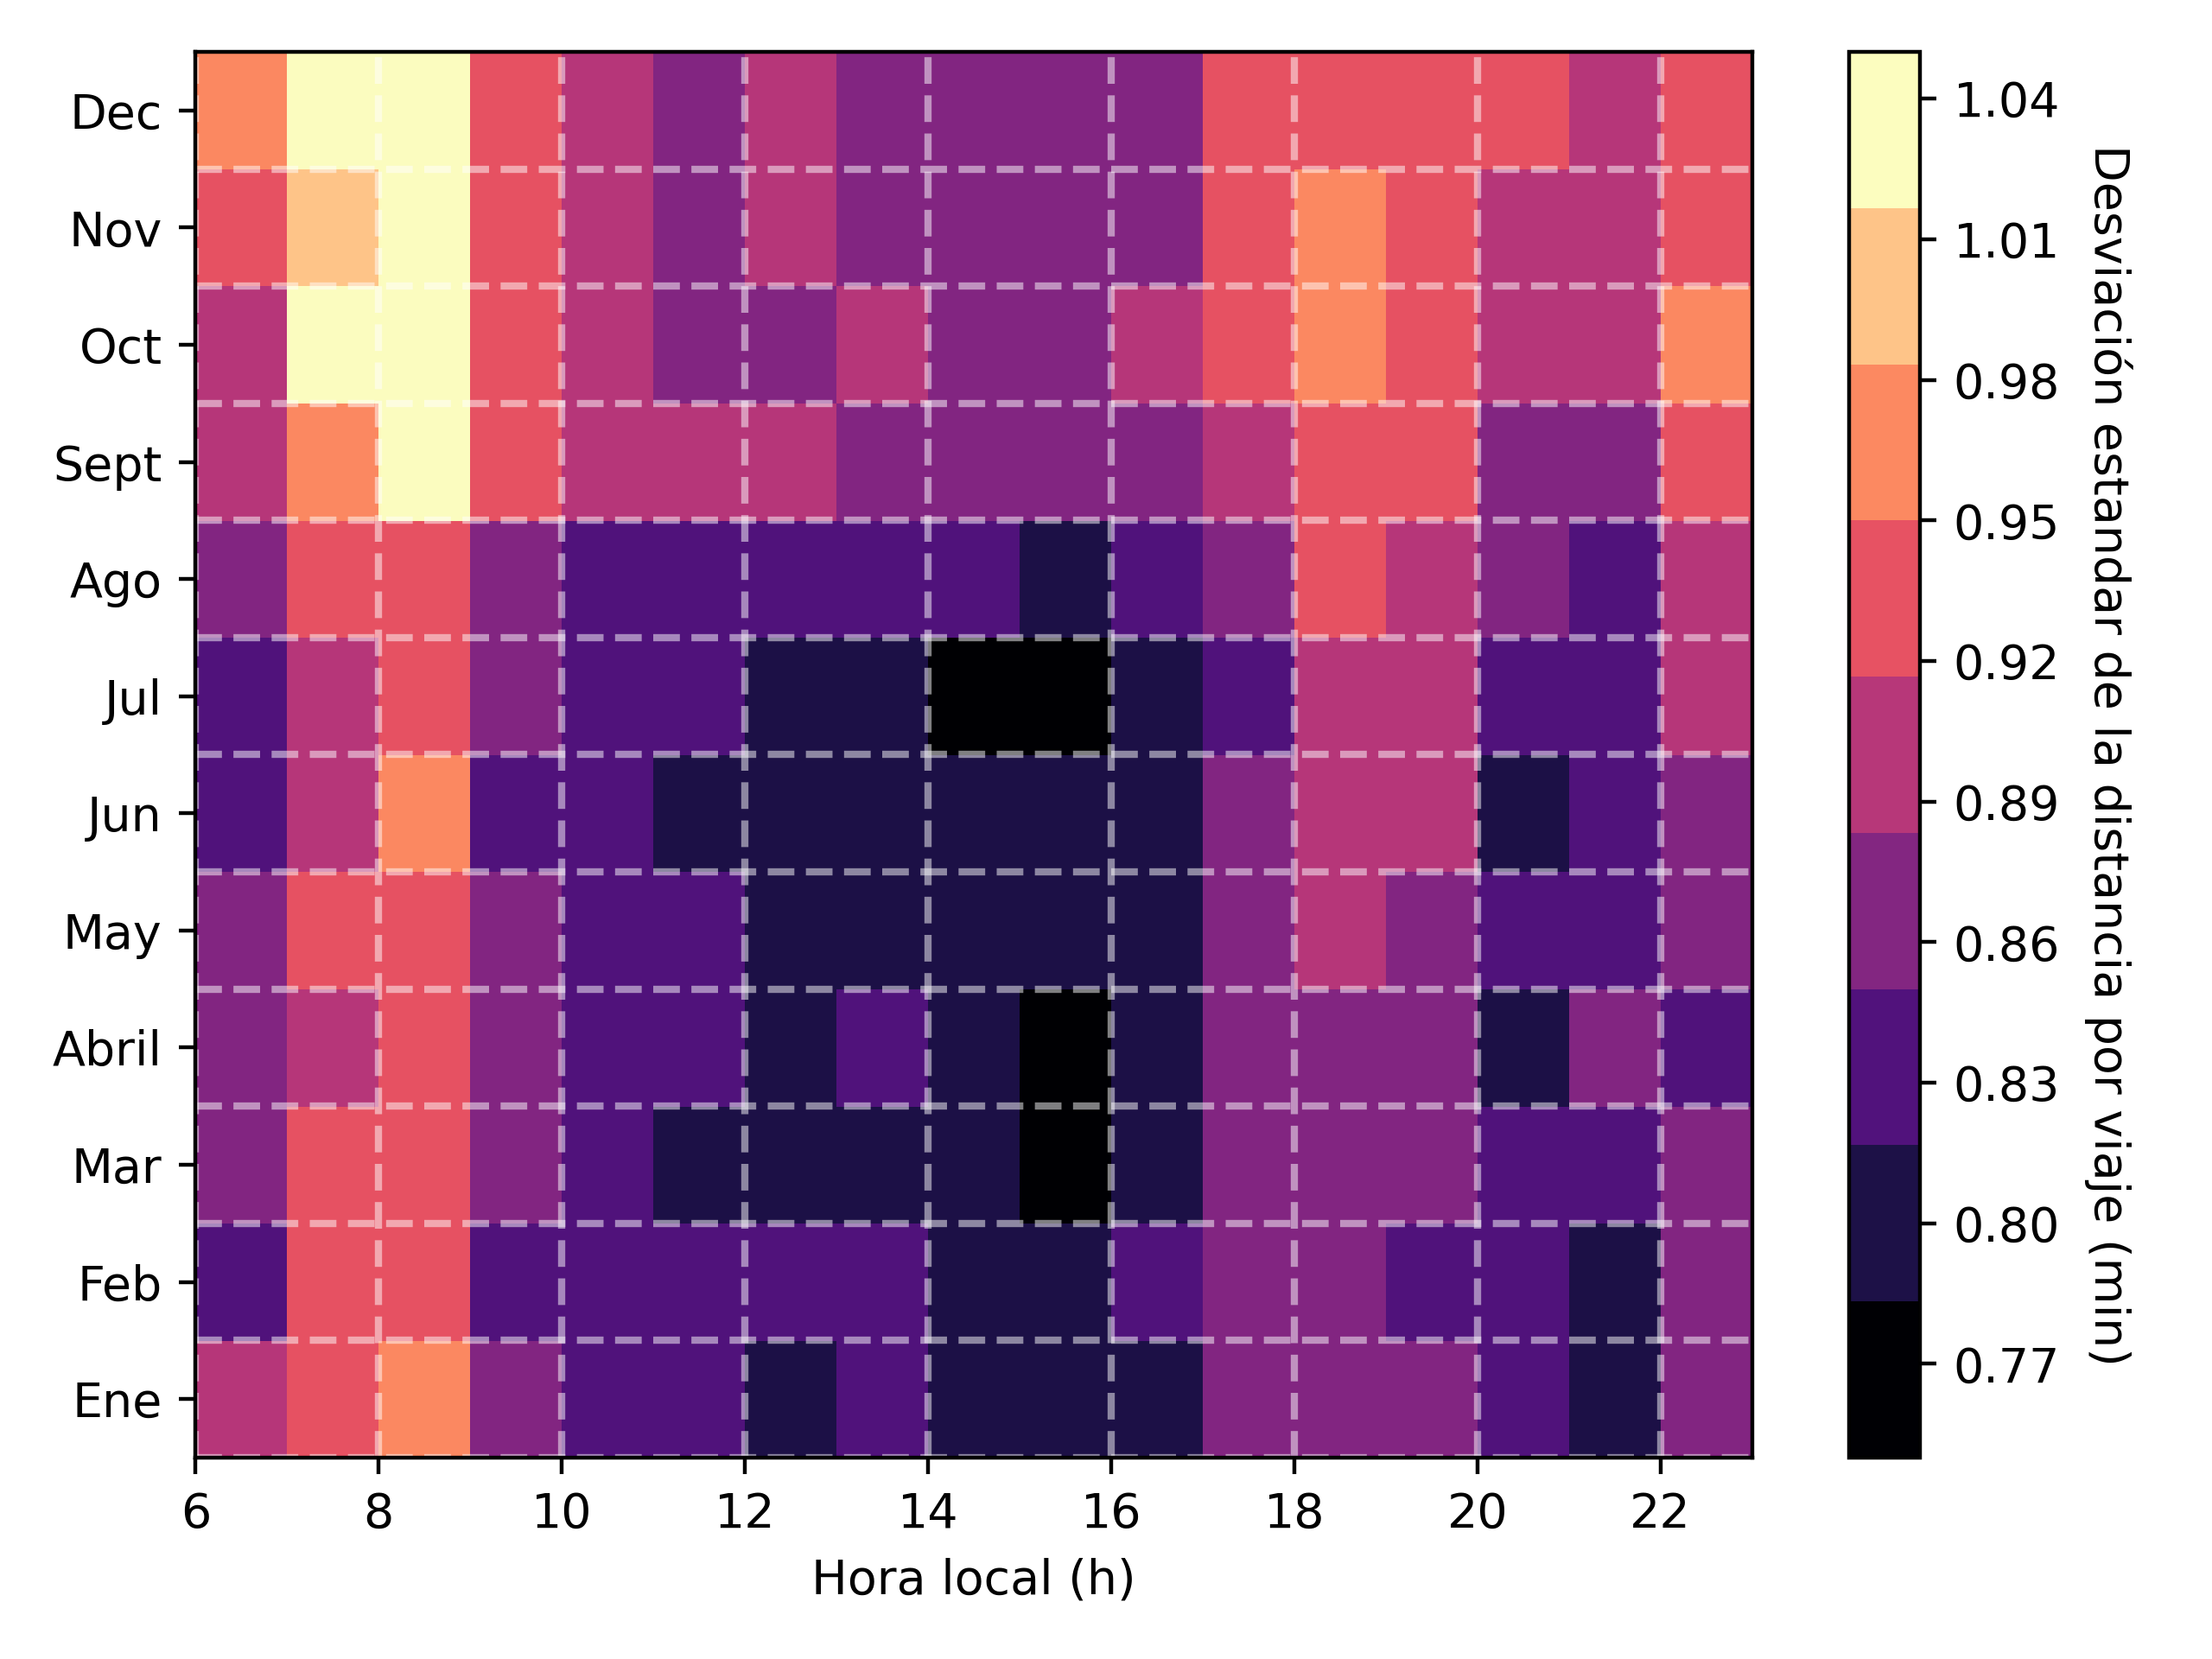
\includegraphics[width=8cm]{Graphics/monthly_hourly_var_distance.png}
        \caption{Desviación estandar mensual de la distancia recorrida.}
        \label{fig:monthly_hourly_var_distance}
    \end{subfigure}
    \caption{Distancia promedio y desviación estandar mensual por hora recorrida por lo usuarios calculadas con las ecuaciones \ref{eq:monthly_hourly_mean_distance} y \ref{eq:monthly_hourly_var_distance}.}
    \label{fig:monthly_hourly_distance}
\end{figure}

Otra manera de abordar los datos es realizando un promedio del día semanal por las horas del día. Esto se obtuvo aplicando la ecuación \ref{eq:daily_hourly_mean_distance} a los datos.

\begin{equation}
    \hat{D}_{d,h} = \frac{1}{n_{(d,h)}} = \sum_{i=1}^{n_{(d,h)}} \hat{D}_{i} \qquad \begin{matrix}
        d=1,2,\dots,7 \\ h=6,7,\dots,23
    \end{matrix} \label{eq:daily_hourly_mean_distance}
\end{equation}

donde $D_i$ y $n_{(d,h)}$ es el conjunto y la cantidad total de viajes realizados para el día de la semana $d$ realizados entre las $h$ y $h+1$ horas respectivamente. De una manera semejante, se calculo la varianza de este conjunto con la ecuación \ref{eq:daily_hourly_var_distance}.

\begin{equation}
    \sigma_{D_{(m,h)}} = \frac{1}{n_{(m,h)}-1} \sum_{i=1}^{n_{(m,n)}} (D_i-\bar{D}_{(d,h)})^2 \qquad \begin{matrix}
        m=1,2,\dots,12 \\ h=6,7,\dots,23
    \end{matrix} \label{eq:daily_hourly_var_distance}
\end{equation}

En la figura \ref{fig:daily_hourly_distance} se muestran los resultados de aplicar las ecuaciones \ref{eq:daily_hourly_mean_distance} y \ref{eq:daily_hourly_var_distance} a los datos de las distancias.

En la figura \ref{eq:daily_hourly_mean_distance} se aprecia que el uso de la bicicleta se incrementa entre semana a las 7:00 horas y 15:00 horas. Existe una disminución de la distancia recorrida entre las 12 y 16 horas, algo que ya se habia previsto en la figura \ref{fig:daily_hourly_mean_distance}. Se presenta en el periodo de las 8 y 10 horas los días domingo, dando indicios que en ese periodo se usan de manera recreativa. Este indicio también nos lo da la figura \ref{fig:daily_hourly_var_distance}, ya que la variación en ese periodo de tiempo es mayor, y esto puede ser debido a que son usadas en diversas actividades. En cambio entre semana la varianza es poca, dando la impresión que los usuarios realizan una actividad semejante como lo es el transporte de un lugar hacia otro.

\begin{figure}[H]
    \centering
    \begin{subfigure}[b]{8cm}
        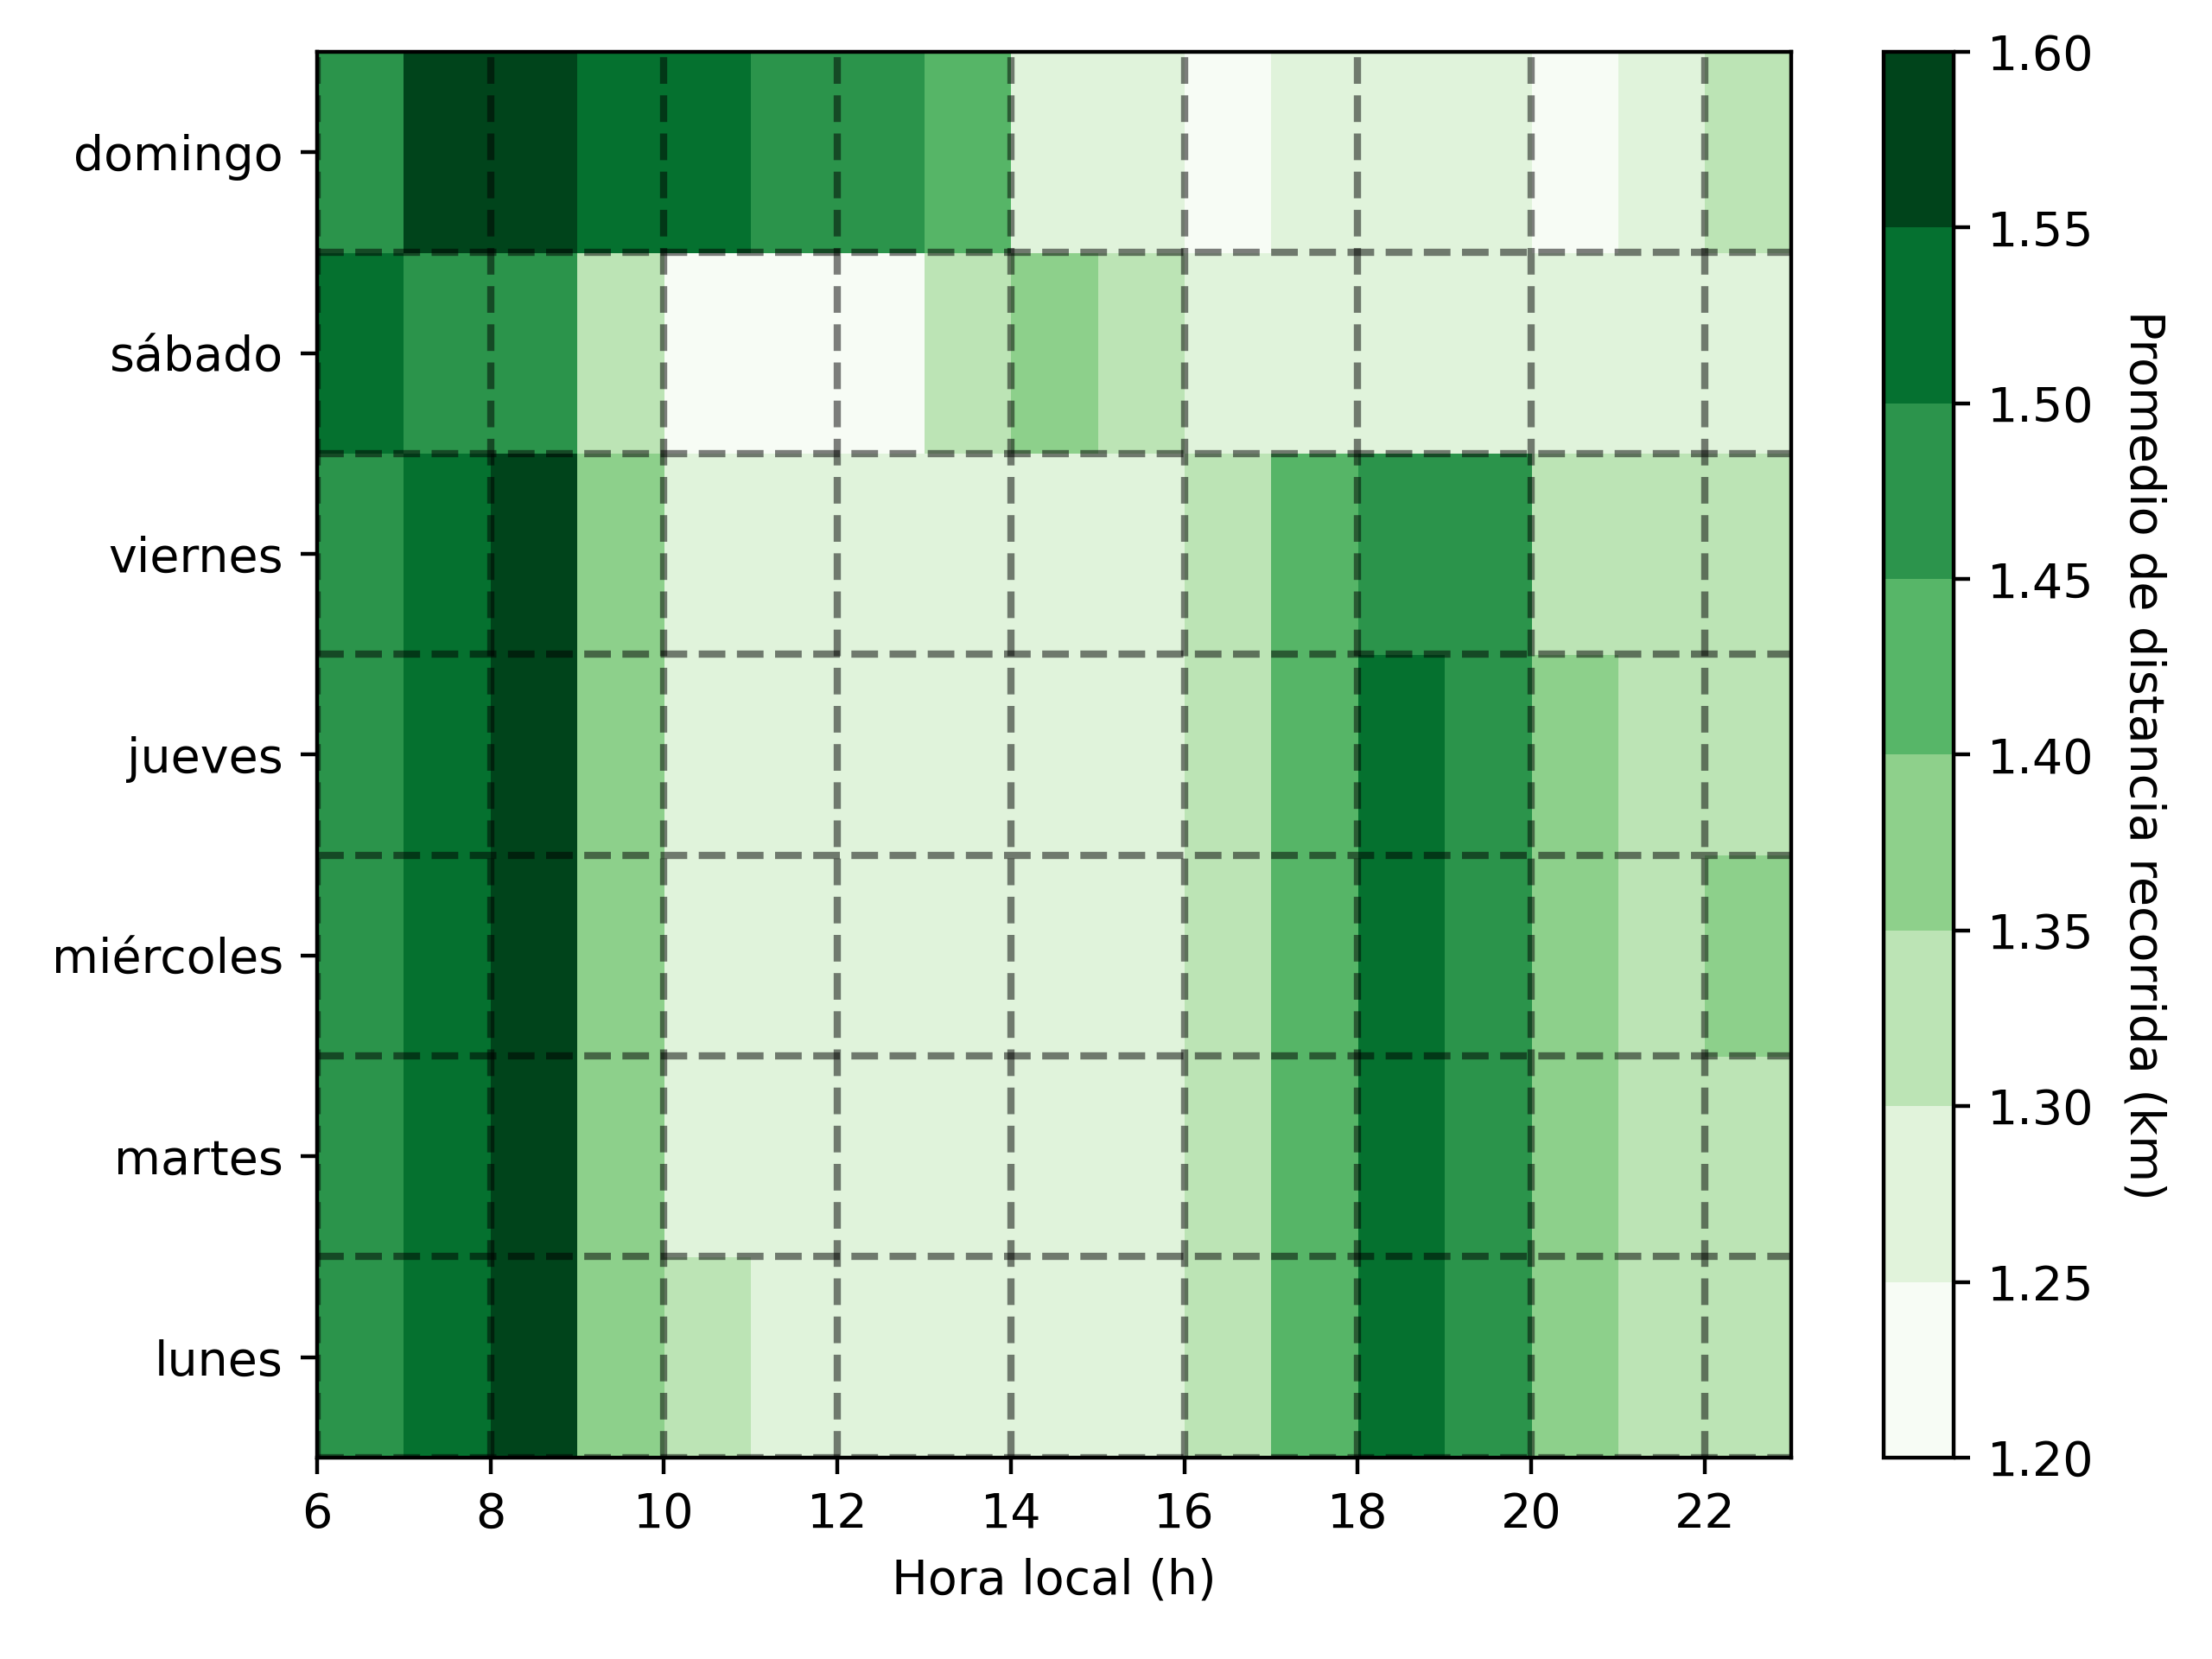
\includegraphics[width=8cm]{Graphics/daily_and_hour_mean_distance.png}
        \caption{Promedio diaria semanal.}
        \label{fig:daily_hourly_mean_distance}
    \end{subfigure}
    \begin{subfigure}[b]{8cm}
        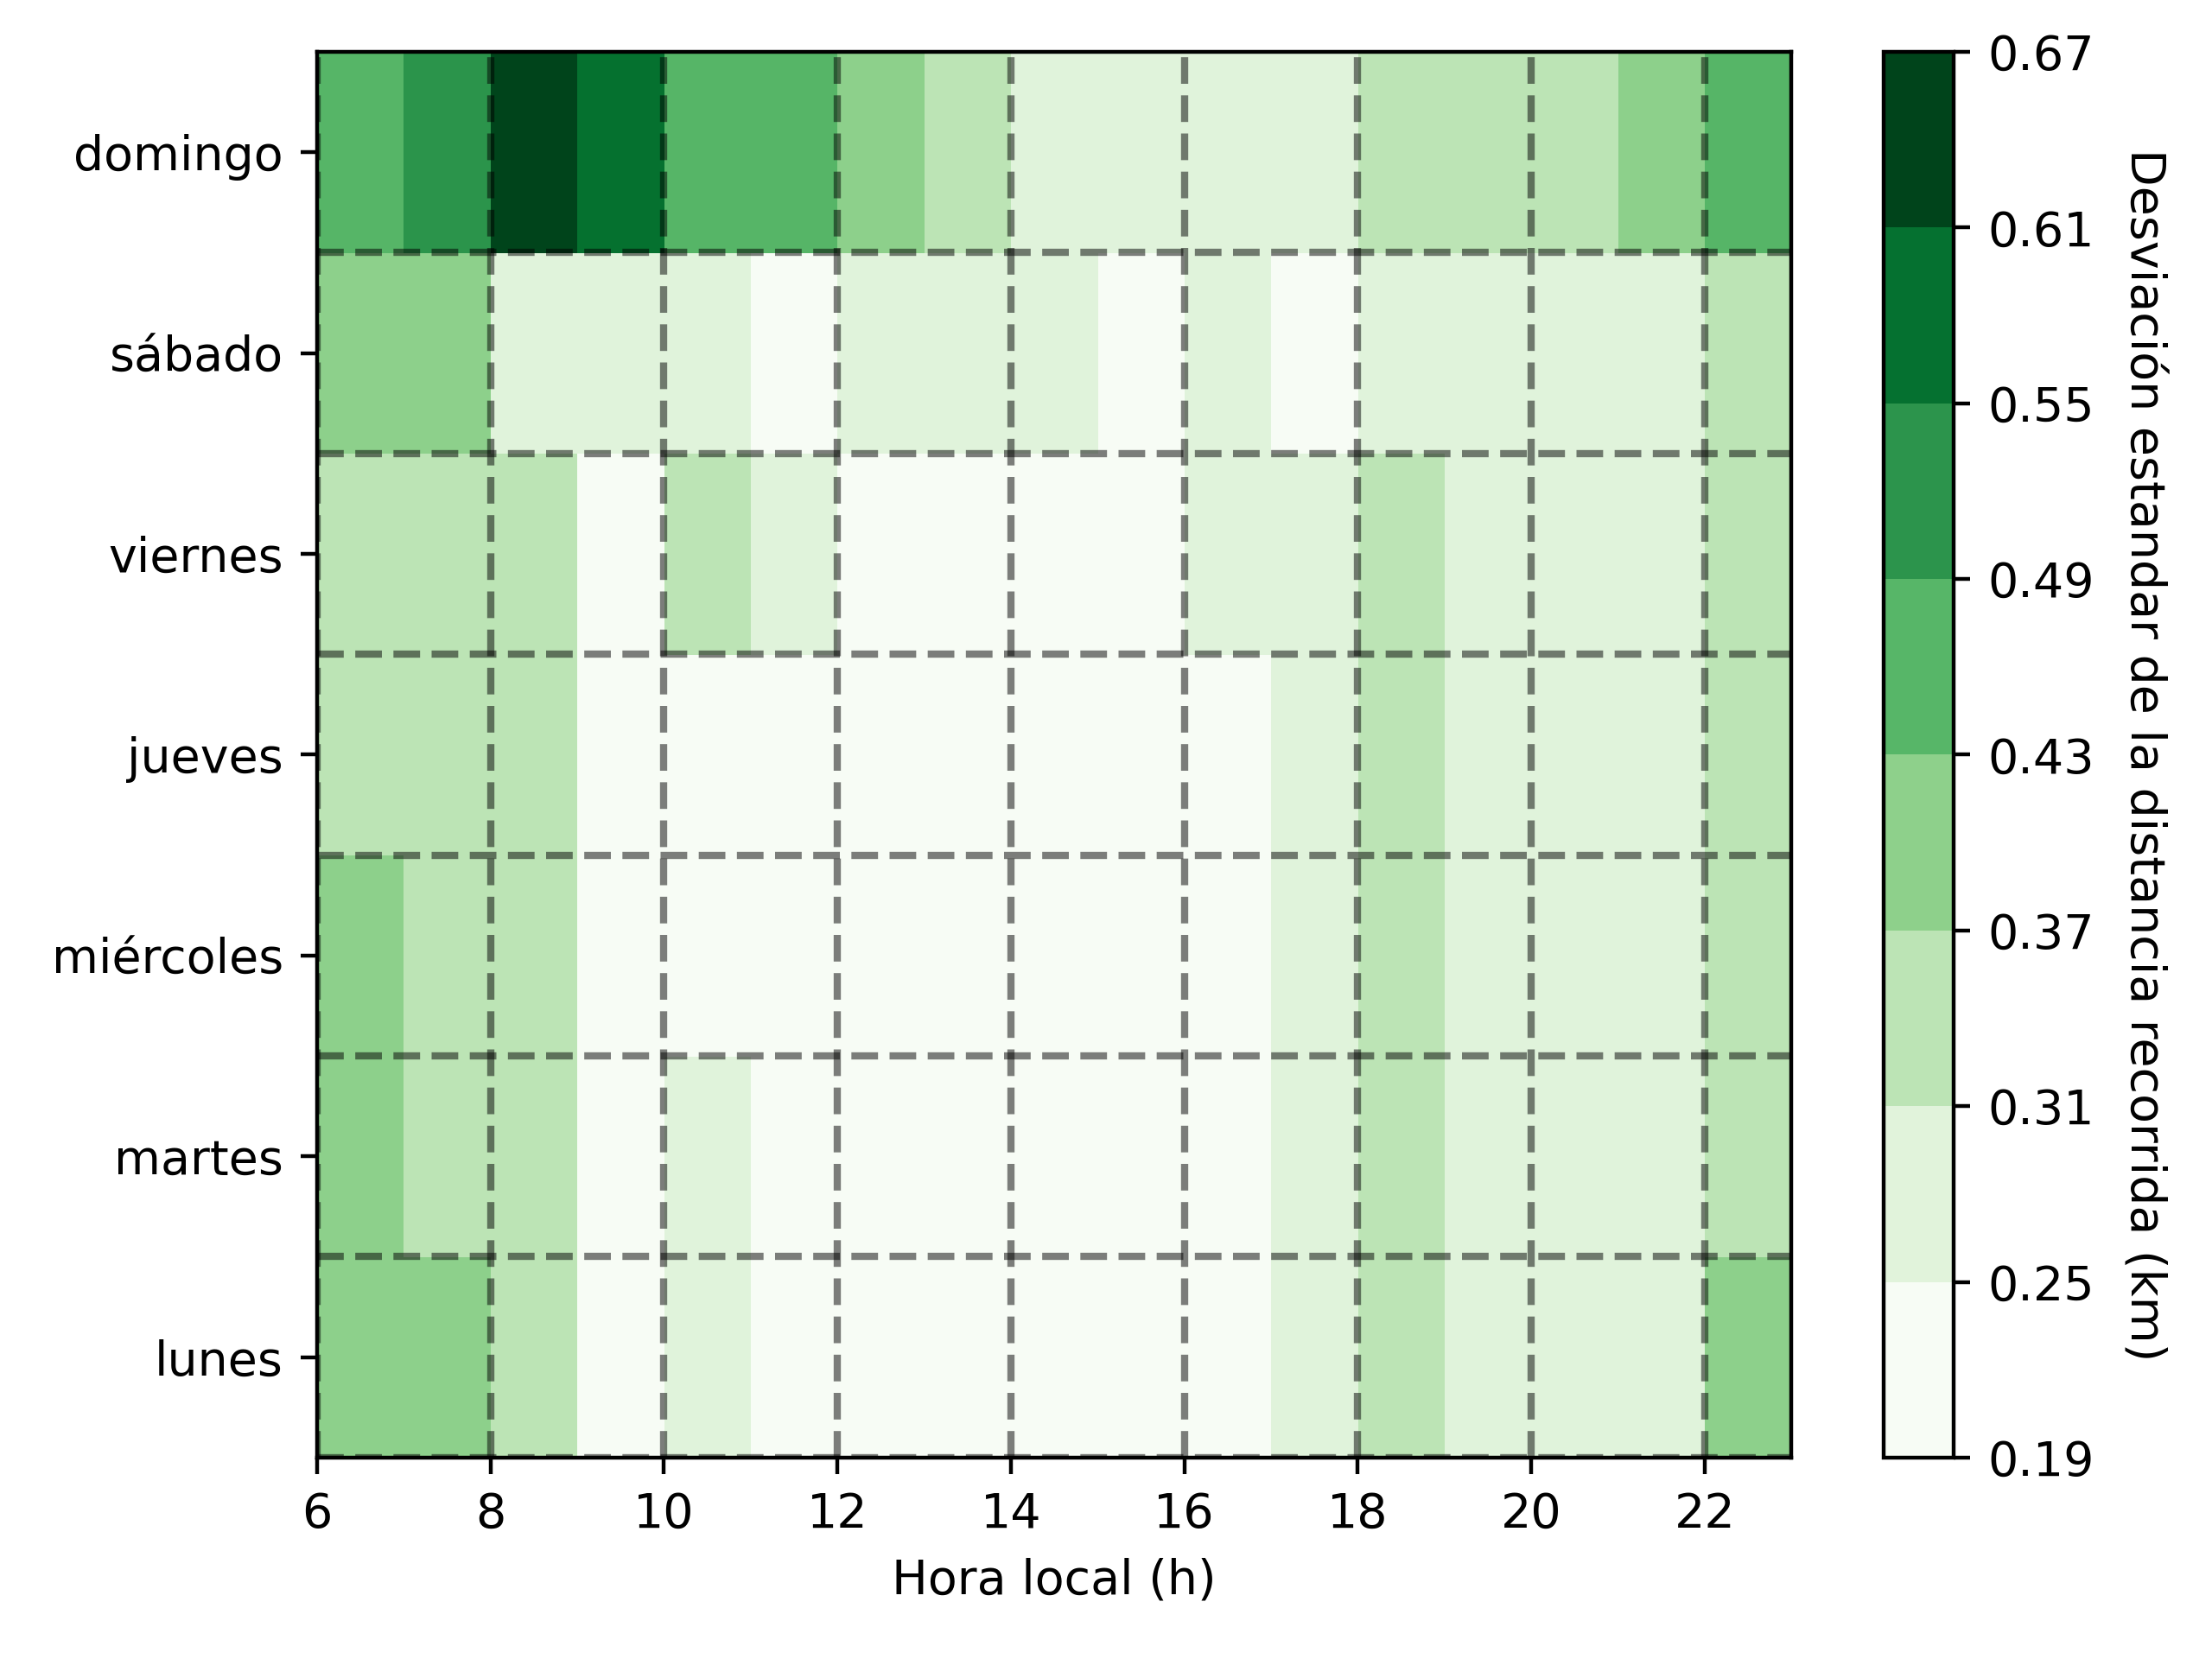
\includegraphics[width=8cm]{Graphics/daily_and_hour_var_distance.png}
        \caption{Desviación estandar diaria semanal.}
        \label{fig:daily_hourly_var_distance}
    \end{subfigure}
    \caption{Distancia promedio y desviación estandar diaria semanal por hora recorrida por lo usuarios calculadas con las ecuaciones \ref{eq:daily_hourly_mean_distance} y \ref{eq:daily_hourly_var_distance}.}
\end{figure}

